
\chapter{Estabilidad de los amplificadores realimentados}\label{estabilidad}
%\def\baselinestretch{1.66}
%\goodbreak
\section{Visión general}

\hspace{10pt} La estabilidad de un amplificador está relacionada en forma directa
con la ubicación de los polos de su función transferencia.

Un amplificador es estable  si todos los polos de su función
transferencia, definida en el plano \emph{s}, poseen parte real
negativa. En forma cualitativa se muestra en la figura \ref{estab1}
la respuesta transitoria al impulso de un amplificador en función de
la posición de sus polos. En las figuras \ref{estab1} a) y b) el
amplificador es estable, en la c) presenta oscilaciones sostenidas y
en las d) y e) su comportamiento es inestable.

En los análisis que se realizarán se parte de la suposición que el
amplificador sin realimentar ($a(s)$) tiene todos sus polos en el
semiplano izquierdo, es decir es estable. Al realimentarlo los polos
de la transferencia total ($A(s)$) se mueven, pudiendo hacerlo hacia
zonas de inestabilidad, es por lo tanto importante el estudio de
estos movimientos para determinar la estabilidad del amplificador.

El esquema básico de un amplificador realimentado es el mostrado en
la figura \ref{estab2}, ya presentado en el capítulo anterior. En
dicha figura se muestra la ecuación de la transferencia realimentada
$A(s)$. Los polos que se mueven del sistema realimentado son las
raíces de la ecuación característica, $ 1 + T(s) = 0 $. Los métodos
que se utilizarán en este capítulo para analizar la estabilidad de
los amplificadores realimentados, se basan en el concepto de
estudiar el comportamiento de las raíces de la mencionada ecuación
característica.



\begin{figure}
	\centering
	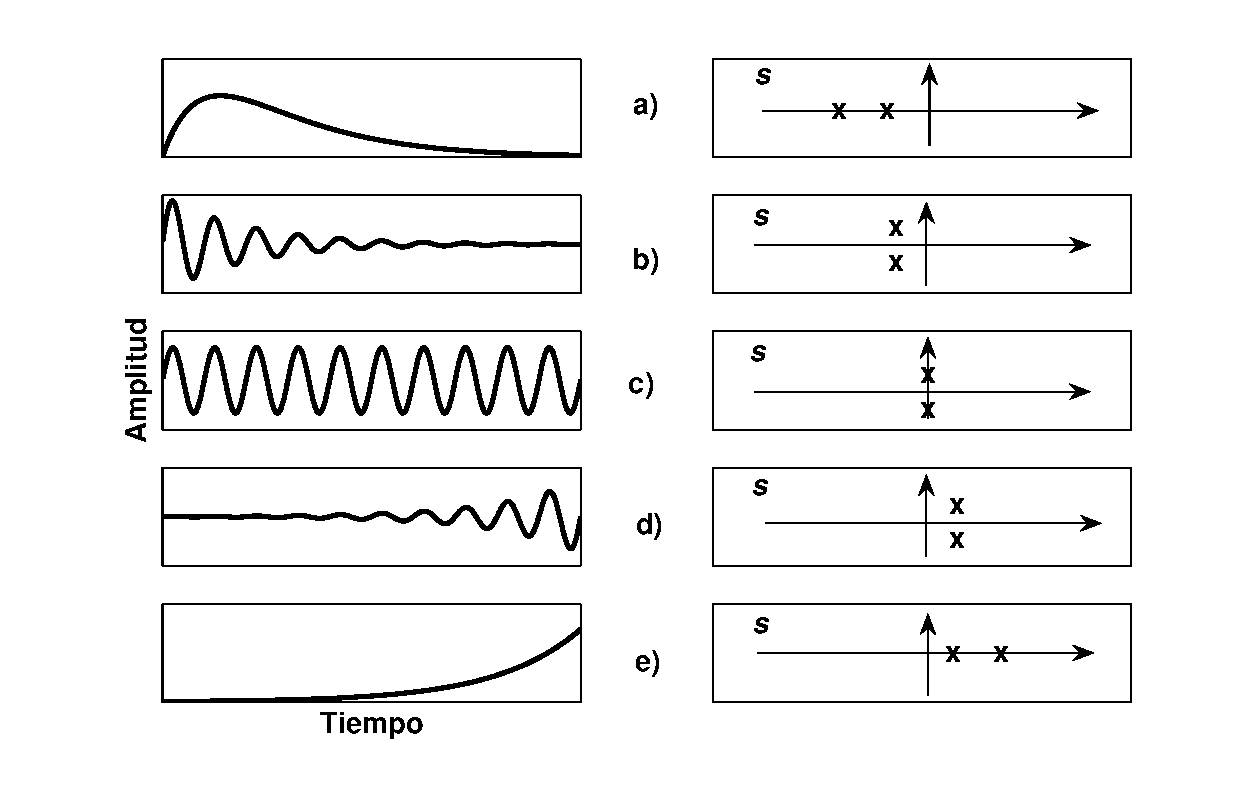
\includegraphics[width=5in]{figuras/estab1.pdf}\\
	\caption{Relación entre la ubicación de los polos y la respuesta transitoria.}\label{estab1}
\end{figure}


\begin{figure}
	\centering
	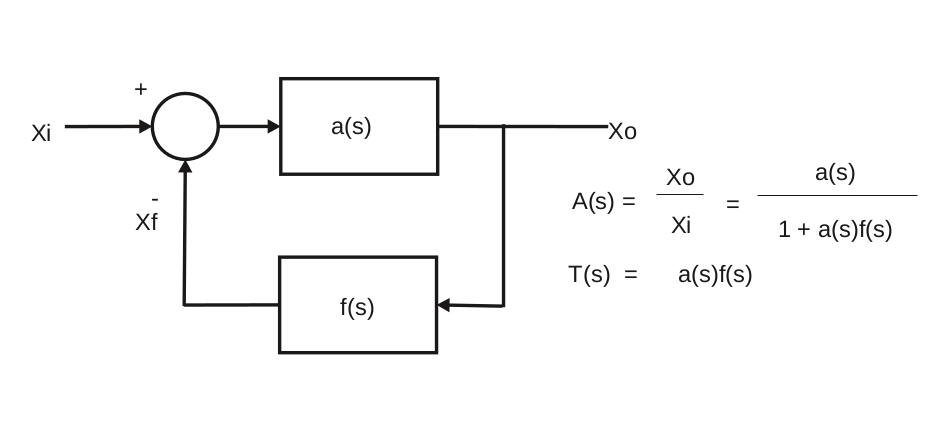
\includegraphics[width=5in]{figuras/estab2.png}\\
	\caption{Esquema teórico de un amplificador realimentado.}\label{estab2}
\end{figure}

\section{Amplificador pasa bajos de un polo}

Partiendo de un amplificador sin realimentar de un polo dado por la
expresión:

	\begin{equation}
		\nonumber
		a(s)=\frac{ \displaystyle a_o}{\displaystyle 1+\frac{s}{\displaystyle w_a}}
	\end{equation}

; donde $a_o$ es la ganancia sin realimentar a bajas frecuencias.
Suponiendo un factor de realimentación $f=f_o$ independiente de la
frecuencia, se llega a la la expresión de la ganancia realimentada:

	\begin{equation}
		\nonumber
		A(s)=\frac{\displaystyle A_o}{\displaystyle (1+  \frac{\displaystyle s}{\displaystyle w_{af}})}
	\end{equation}



En esta expresión $A_o=\frac{\displaystyle a_o}{\displaystyle
	(1+T_o)}$ es la ganancia realimentada a bajas frecuencia, $T_o=a_o
f_o$ es la ganancia de lazo a bajas frecuencias y $w_{af}=w_a
(1+T_o)$ es el polo del amplificador realimentado.

En la figura \ref{estab3} a) se muestra en el plano \emph{s} el
lugar geométrico del polo del sistema en función de $T_o$; en ella
se ve que a medida que aumenta el factor de realimentación $f_o$ (y
por lo tanto $T_o$) el polo se mueve hacia la izquierda, siendo el
sistema incondicionalmente estable. En la figura \ref{estab3} b) se
muestra el diagrama de Bode de amplitud de los sistemas con y sin
realimentación, se deduce fácilmente que en este caso el producto
ganancia por ancho de banda ($a_o w_a=A_o w_{af}$) se mantiene
constante.

\begin{figure}
	\centering
	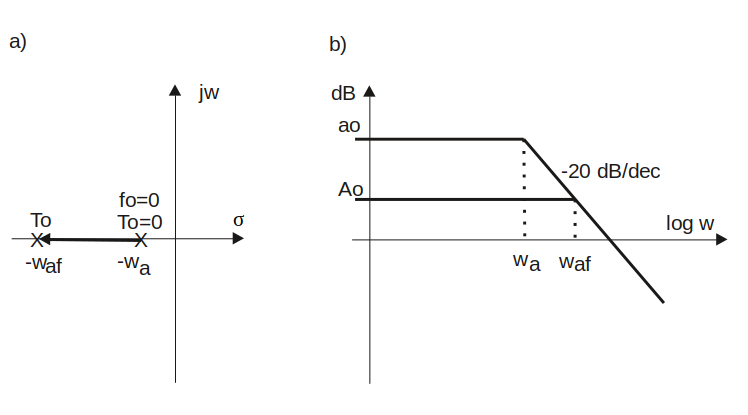
\includegraphics[width=5in]{figuras/estab3.png}\\
	\caption{Amplificador pasa bajos de un polo. a) Movimiento del polo en el plano \emph{s} en función de $T_o$, b) Diagrama de amplitud de Bode.}\label{estab3}
\end{figure}

\section{Amplificador pasa altos de un polo}

\hspace{10pt} Haciendo un análisis similar al del punto anterior, se parte de un
amplificador pasa altos de un polo sin realimentar:

	\begin{equation}
		\nonumber
		a(s)=\frac{\displaystyle a_o \frac{\displaystyle s}{\displaystyle w_a}}{\displaystyle 1+\frac{\displaystyle s}{\displaystyle w_a}}
	\end{equation}

, con un factor de realimentación $f=f_o$, llegando a un
amplificador realimentado,
	\begin{equation}
		\nonumber
		A(s)=\frac{\displaystyle A_o \frac{\displaystyle s}{\displaystyle w_{af}}}{\displaystyle 1+\frac{\displaystyle s}{\displaystyle w_{af}}}
	\end{equation}
; con $A_o=\frac{\displaystyle a_o}{\displaystyle (1+T_o)}$ y
$w_{af}=\frac{\displaystyle w_a}{\displaystyle 1+T_o}$.

En la figura \ref{estab4} a) se muestra en el plano \emph{s} el
lugar geométrico del polo del sistema en función de $T_o$; en ella
se ve que a medida que aumenta el factor de realimentación $f_o$ (y
por lo tanto $T_o$) el polo se mueve hacia la derecha acercándose al
cero, siendo el sistema estable. En la figura \ref{estab4} b) se
muestra el diagrama de Bode de amplitud de los sistemas con y sin
realimentación.
\begin{figure}
	\centering
	
\includegraphics[width=5in]{figuras/estab4.png}\\
	\caption{Amplificador pasa altos de un polo. a) Movimiento del polo en el plano \emph{s} en función de $T_o$, b) Diagrama de amplitud de Bode.}\label{estab4}
\end{figure}

\section{Amplificador de dos polos}

\hspace{10pt} Partiendo de un amplificador sin realimentar de dos polos:

	\begin{equation}
		\nonumber
		a(s)=\frac{\displaystyle a_o}{\displaystyle (1 + \frac{\displaystyle s}{\displaystyle w_a})(1 + \frac{\displaystyle s}{\displaystyle w_b})}
	\end{equation}

y suponiendo, como en los casos anteriores, $f(s)=f_o$, se llega a
la siguiente expresión de la ganancia realimentada:
	\begin{equation}
		\nonumber
		A(s)=\frac{\displaystyle a_o}{\displaystyle (1 + \frac{\displaystyle s}{\displaystyle w_a})(1 + \frac{\displaystyle s}{\displaystyle w_b})+a_o f_o}=\frac{\displaystyle A_o}{\displaystyle \frac{\displaystyle s^2}{\displaystyle w_a w_b (1+T_o)} + \frac{\displaystyle s ( w_a+w_b)}{\displaystyle w_a w_b (1+T_o)} + 1}
	\end{equation}

La expresión resultante, un sistema de 2° orden, puede llevarse a la
siguiente forma:

	\begin{equation}
		\nonumber
		A(s)=\frac{\displaystyle A_o}{\frac{\displaystyle s^2}{\displaystyle w_o^2} + \frac{\displaystyle s}{\displaystyle Q  w_o} + 1}
	\end{equation}

Donde $A_o=\frac{\displaystyle a_o}{\displaystyle 1+T_o}$,
$w_o=\sqrt{w_a w_b (1 + T_o)}$ y $Q = \frac{\displaystyle
	w_o}{\displaystyle w_a + w_b}$. Resolviendo la ecuación
$\frac{\displaystyle s^2}{\displaystyle w_o^2} + \frac{\displaystyle
	s}{\displaystyle Q w_o} + 1 = 0$ se obtienen los polos del
amplificador realimentado dados por la expresión:

	\begin{eqnarray}
		\nonumber
		-\frac{\displaystyle w_o}{\displaystyle 2 Q}(1 \pm \sqrt{(1-4 Q^2)}) & \quad \quad & si \quad Q \leq  \frac{\displaystyle 1}{\displaystyle 2} \\
		\nonumber
		-\frac{\displaystyle w_o}{\displaystyle 2 Q}(1 \pm j \sqrt{(4 Q^2-1)}) & \quad \quad & si \quad Q >  \frac{\displaystyle 1}{\displaystyle 2} \\
		\nonumber
	\end{eqnarray}


En la figura \ref{estab5} se ve el lugar geométrico de los polos del
amplificador en función de $T_o$ (o en función de $Q$). Este gráfico
revela que un amplificador de estas características es
incondicionalmente estable; sin embargo a medida que se aumenta el
grado de realimentación los polos del sistema aumentan su parte
imaginaria, manteniendo su parte real constante. En estas
circunstancias la respuesta en frecuencia y la respuesta transitoria
pueden no ser las adecuadas e incluso la cercanía de los polos del
sistema al eje imaginario puede hacer que efectos de segundo orden
no contemplados en el modelo original lleven al amplificador a zonas
de inestabilidad.
\begin{figure}
	\centering
	
\includegraphics[width=5in]{figuras/estab5.png}\\
	\caption{Amplificador de dos polos. Movimientos de los polos en función de $T_o$.}\label{estab5}
\end{figure}

En la figura \ref{estab6} se muestra en forma cualitativa como la
respuesta en frecuencia puede presentar sobrepicos en función de la
cantidad de realimentación. En dicha figura $w_x$ es la frecuencia a
la que se produce el sobrepico. Se demuestra hallando el máximo del
módulo de la transferencia, que el sobrepico existe para $Q >
\frac{\displaystyle \sqrt{2}}{\displaystyle 2}$ en $w_x =w_o
\sqrt{1-\frac{\displaystyle 1}{\displaystyle 2 Q^2}}$; y que el
valor de dicho sobrepico es: $\mid \frac{\displaystyle
	A(jw_x)}{\displaystyle A_o} \mid = \frac{\displaystyle 2
	Q^2}{\displaystyle \sqrt{4 Q^2 - 1}}$.
\begin{figure}
	\centering
	
\includegraphics[width=5in]{figuras/estab6.png}\\
	\caption{Sobrepico de la ganancia en un amplificador de dos polos.}\label{estab6}
\end{figure}

La respuesta transitoria al escalón, muestra también sobreimpulsos
para $Q > \frac{\displaystyle 1}{\displaystyle 2}$. En la figura
\ref{estab7} se muestras un ejemplo para $Q=2$. La expresión de la
respuesta transitoria al escalón $V_i(t)= V_e \mu (t)$ es:

	\begin{equation}
		\nonumber
		\frac{\displaystyle V_o(t)}{\displaystyle V_e}=1 - \sqrt{\frac{\displaystyle 4 Q^2}{\displaystyle 4 Q^2-1}} e^{-\alpha t}\sin{(\beta t + \arccos{\frac{\displaystyle 1}{\displaystyle 2 Q}})}
	\end{equation}

El primer sobreimpulso tiene un valor porcentual dado por: $SI \% =
e^{-{\frac{\displaystyle \pi}{\displaystyle \sqrt{4 Q^2-1}}}}\times
100$.

\begin{figure}
	\centering
	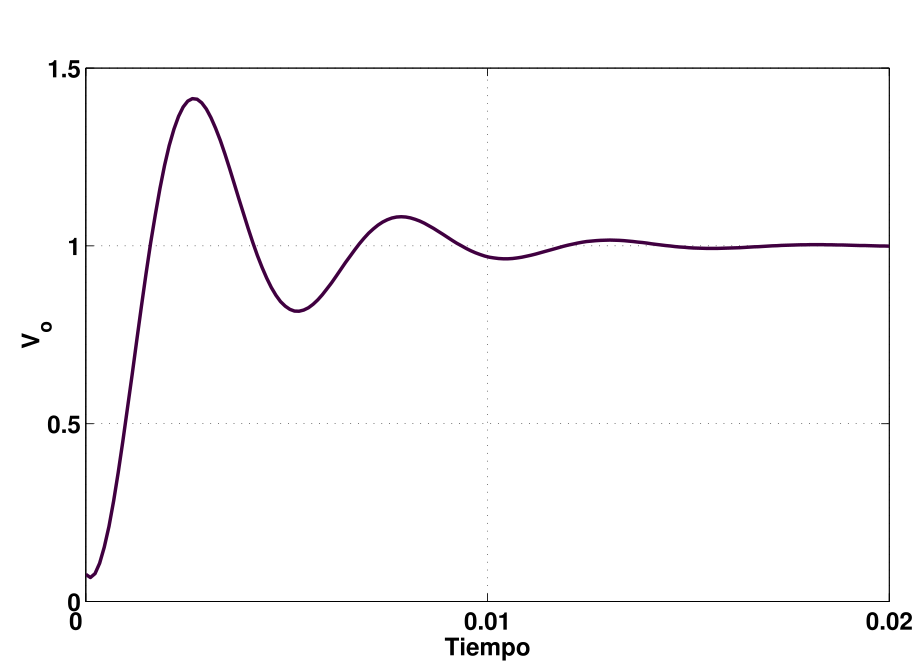
\includegraphics[width=5in]{figuras/estab7.png}\\
	\caption{Respuesta al escalón para un amplificador de dos polos con $Q=2$.}\label{estab7}
\end{figure}

\section{Criterio de estabilidad de Bode}

\hspace{10pt} Si bien en cada amplificador en particular se pueden hacer análisis
similares a los realizados en los puntos anteriores, es útil contar
con métodos más generales para analizar la estabilidad de los
amplificadores realimentados. Uno de los métodos más utilizados es
el denominado criterio de Bode, que utiliza los diagramas de Bode de
amplitud y fase de la transferencia de lazo $T(jw)$. Este método
deriva de uno más general, el método de Nyquist; la demostración
matemática de estos dos métodos pueden consultarse en la
bibliografía recomendada. Aquí daremos una visión
intuitiva del método de Bode, partiendo del concepto fundamental de
utilizar la ecuación característica ($1+T(s)=0$); y basándonos en un
caso particular, un amplificador de tres polos.

Partiremos por lo tanto de un amplificador sin realimentar de tres
polos, la expresión de dicha transferencia es:

	\begin{equation}
		\nonumber
		a(s)=\frac{\displaystyle a_o}{\displaystyle (1+\frac{\displaystyle s}{\displaystyle w_a})(1+\frac{\displaystyle s}{\displaystyle w_b})(1+\frac{\displaystyle s}{\displaystyle w_c})}
	\end{equation}

Supondremos que el factor de realimentación no depende de la
frecuencia ($f(s)=f_o$). La transferencia del amplificador
realimentado será entonces:

	\begin{equation}
		\nonumber
		A(s)=\frac{\displaystyle a(s)}{\displaystyle 1+a(s)f(s)}=\frac{\displaystyle A_o}{\displaystyle \frac{\displaystyle s^3}{\displaystyle (1+T_o)w_a w_b w_c} + \frac{\displaystyle s^2 (w_a+w_b+w_c)}{\displaystyle (1+T_o)w_a w_b w_c}+\frac{\displaystyle s(w_a w_b+w_a w_c+w_b w_c)}{\displaystyle (1+T_o)w_a w_b w_c}+1}
	\end{equation}

, con $T_o=a_o f_o$ y $A_o=\frac{\displaystyle a_o}{\displaystyle
	1+T_o}$.

Si trazamos el lugar geométrico de las raíces del polinomio del
denominador en la expresión anterior (los polos del amplificador
realimentado), en función de $T_o$; obtendremos un resultado como el
visto en la figura \ref{estab8}. En esta figura se ve que los polos
$w_a$ y $w_b$, a medida que aumenta $T_o$, tienden a juntarse en
primera instancia para luego convertirse en complejos conjugados con
parte real negativa (estable) para $T_o < T_{oc}$ y parte real
positiva (inestable) para $T_o > T_{oc}$. El caso límite se da para
el valor crítico $T_o=T_{oc}$ en donde los polos son imaginarios
puros (inestable con oscilaciones sostenidas). Es de notar que el
polo $w_c$ se mueve hacia la izquierda a medida que crece $T_o$.

Apoyándonos intuitivamente en la figura \ref{estab8} podemos decir
que como el lugar geométrico graficado es el de $T(s)=-1$;
particularmente $T(jw)=-1$ se dará para $T_o=T_{oc}$. Por lo tanto
el gráfico de Bode de un amplificador en condiciones de oscilaciones
sostenidas deberá necesariamente tomar el valor $-1$ a una
determinada frecuencia que llamaremos $w_{osc}$.
\begin{figure}
	\centering
	
\includegraphics[width=5in]{figuras/estab8.png}\\
	\caption{Amplificador de tres polos.}\label{estab8}
\end{figure}

Se utilizará un amplificador con $a_o=1000$, $w_a=1$, $w_b=10$ y
$w_c=100$ para cuantificar el análisis. En la figura \ref{estab9} se
grafica el diagrama de Bode de $T(jw)$ del amplificador para tres
casos distintos de realimentación: a) $f_o=0,1$ ($T_o=100$), b)
$f_o=0,01$ ($T_o=10$) y c) $f_o=1$ ($T_o=1000$). El diagrama de fase
es el mismo para los tres casos debido a que el factor de
realimentación no depende de la frecuencia. Se ve que el caso a)
corresponde al $T_{oc}$ ya que a la frecuencia $w_{osc}$ la amplitud
vale $0 dB$ y la fase $-180°$, por lo tanto es un caso de
inestabilidad con oscilaciones sostenidas. El caso b) es un caso
estable ya que $T_o < T_{oc}$, para este caso se puede ver que a la
frecuencia en que la amplitud pasa por $0 dB$ la fase aún no llega
$-180°$. Contrariamente en el caso c), caso inestable con $T_o >
T_{oc}$, la fase excede a $-180°$ a la frecuencia de $0 dB$.

Si nombramos como $w_{0dB}$ a la frecuencia en que la amplitud de
$T(jw)$ medida en decibeles vale $0 dB$; se puede definir entonces
al \textbf{margen de fase}:

	\begin{equation}
		\nonumber
		M_\Phi=180°+\Phi(T(jw_{0dB}))
	\end{equation}

Es decir el ángulo que le falta a $\Phi(T(jw_{0dB}))$ para llegar a
$-180°$.

En forma similar si nombramos a $w_{-180°}$ a la frecuencia en que
la fase de $T(jw)$ pasa por $-180°$; se puede definir el
\textbf{margen de ganancia} como:

	\begin{equation}
		\nonumber
		M_G=-20 \log(|T(jw_{-180°}|)
	\end{equation}

Es decir cuanto por debajo de $0dB$ está $|T(jw)|$ cuando la fase es
$-180°$.

Generalizando se puede afirmar que para que los amplificadores
realimentados sean estables, los márgenes de fase y ganancia deben
ser positivos. En los casos en que dichos márgenes no estén
unívocamente determinados, es aconsejable utilizar otros métodos
complementarios (Nyquist, lugar de raíces, etc) para interpretar los
resultados adecuadamente.
%\begin{figure}
%    \centering
%    
\includegraphics[width=5in]{estab9}\\
%    \caption{Criterio de Bode.}\label{estab9}
%\end{figure}

\section{Relación entre el margen de fase y la respuesta en frecuencia}

\hspace{10pt} Cuando se analizó el amplificador de dos polos se mostró que la
respuesta en frecuencia del amplificador realimentado podía
presentar sobrepicos, y que éstos aumentaban a medida que se
incrementaba $T_o$, o visto de otra manera cuando se incrementaba el
parámetro $Q$. De lo desarrollado en ese punto se puede deducir que
$Q=\sqrt{(1+T_o) m}$ siendo $m=\frac{\displaystyle w_a
	w_b}{\displaystyle (w_a+w_b)^2}=\frac{\displaystyle
	\frac{\displaystyle w_a}{\displaystyle w_b}}{\displaystyle
	(1+\frac{\displaystyle w_a}{\displaystyle w_b})^2}$. En el caso de
dos polos se puede obtener, con un desarrollo matemático sencillo
aunque algo extenso, la expresión del margen de fase en función de
$Q$ con el factor $m$ como parámetro, ésta es:

	\begin{equation}
		\nonumber
		M_\Phi=\arctan(\frac{\displaystyle (\sqrt{(Q^2-m)^2-m+0,25}+m-0,5)^{\frac{\displaystyle 1}{\displaystyle 2}}}{\displaystyle \sqrt{(Q^2-m)^2-m+0,25}-0,5})
	\end{equation}

En la figura \ref{estab10} se muestra el $M_\Phi$ de un amplificador
de dos polos en función de $Q$ para tres valores del parámetro $m$,
viendo que a medida que aumenta $Q$ el margen de fase disminuye;
coincidiendo con un aumento en el sobrepico en la ganancia según lo
ya explicado.

\begin{figure}
	\centering
	
\includegraphics[width=5in]{figuras/estab9.png}\\
	\caption{Criterio de Bode.}\label{estab9}
\end{figure}

\begin{figure}
	\centering
	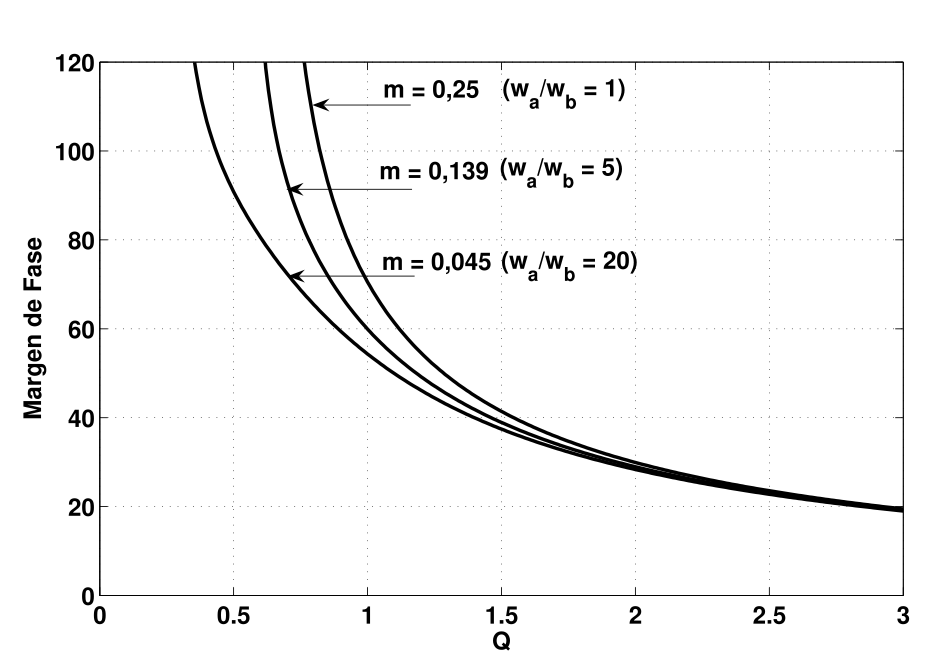
\includegraphics[width=5in]{figuras/estab10.png}\\
	\caption{Margen de fase en función de $Q$ para un amplificador realimentado de dos polos, utilizando el factor $m$ como parámetro.}\label{estab10}
\end{figure}

El caso anterior es un ejemplo particular de la influencia del
margen de fase en la respuesta en frecuencia de un amplificador
realimentado. En forma más general se puede decir que los
amplificadores realimentados están normalmente diseñados con un
margen de fase de al menos $45°$; debido al pronunciado sobrepico
que presentan sus respuestas con márgenes de fase menores al límite
práctico enunciado.

Para comprender mejor estas afirmaciones utilizaremos un
amplificador en el que supondremos que posee una ganancia de lazo a
bajas frecuencias $T_o\gg1$  y un factor de realimentación $f_o$
independiente de la frecuencia. En estas circunstancias la ganancia
realimentada de baja frecuencia será $A_o \simeq \frac{\displaystyle
	1}{\displaystyle f_o}$. Si denominamos $w_1$ a la frecuencia a la
que $\mid T(jw_1) \mid=1$, podemos expresar a  $T(jw_1)=e^{j
	\Phi(T(jw_1))}$, es decir un número complejo con módulo $1$ y fase
$\Phi(T(jw_1))=-180°+M\Phi$.

Como $\mid T(jw_1) \mid=\mid a(jw_1) \mid \mid f_o \mid = 1$,
podemos expresar que $\mid a(jw_1) \mid = \frac{\displaystyle
	1}{\displaystyle f_o}$. De este modo la ganancia realimentada a la
frecuencia $w_1$ será:
	\begin{equation}
		\nonumber
		\mid A(jw_1) \mid = \frac{\displaystyle \mid a(jw_1) \mid}{\displaystyle \mid 1 + T(jw_1) \mid} = \frac{\displaystyle \frac{\displaystyle 1}{\displaystyle f_o}}{\displaystyle \mid 1 + e^{j(-180°+M\Phi)} \mid}
	\end{equation}

Para dar algunos ejemplos  numéricos de esta expresión si el
$M\Phi=30°$, $\mid A(jw_1) \mid \simeq \frac{\displaystyle
	1,93}{\displaystyle f_o}$ (sobrepico del 93\% en $w=w_1$); si
$M\Phi=45°$, $\mid A(jw_1) \mid \simeq \frac{\displaystyle
	1,31}{\displaystyle f_o}$; si $M\Phi=60°$, $\mid A(jw_1) \mid \simeq
\frac{\displaystyle 1}{\displaystyle f_o}$ (sin sobrepico). Para
márgenes de fase superiores a $60°$ no se presentan sobrepicos a la
frecuencia $w_1$.

\section{Compensación}

\hspace{10pt} Volviendo al ejemplo de la figura \ref{estab9}; vemos que el caso a)
($M\Phi=0$) y el caso c) ($M\Phi<0$) son inestables. Compensar a
estos amplificadores es actuar sobre sus transferencias de lazo
$T(s)$ de modo que se vuelvan estables. El método más sencillo
podría ser disminuir la cantidad de realimentación $f_o$ y por
ejemplo pasar al caso b) en donde el $M\Phi>0$. Esta solución puede
no ser aceptable, ya que al disminuir $f_o$, aumenta necesariamente
el valor de la ganancia realimentada a frecuencias bajas $A_o$.

En general compensar un amplificador realimentado es actuar sobre la
ganancia de lazo $T(s)$ de modo de obtener un margen de fase
determinado, sin modificar la ganancia realimentada a frecuencias
bajas o medias $A_o$.

Por los motivos de respuesta en frecuencia explicados en el punto
anterior; se suele considerar desde el punto de vista práctico que
los amplificadores deberán tener un margen de fase de al menos
$45°$.

Como dijimos antes, para compensar un amplificador se debe actuar
sobre $T(s)$. En algunos casos, sin embargo, se dispone de un
amplificador sin realimentar $a(s)$ de respuesta conocida al que se
va utilizar en distintas aplicaciones con factores de realimentación
$f_o$ diferentes. Bajo estas circunstancias se suele actuar
directamente sobre $a(s)$, suponiendo realimentación unitaria
($f_o=1)$, compensándolo para tener un margen de fase de $45°$. Es
de notar que al ser éste el peor caso desde el punto de vista de la
estabilidad, la compensación estará asegurada para cualquier otro
caso. Esta estrategia es la que se sigue en general con los
amplificadores operacionales.

\subsection{Compensación por polo dominante}\label{ejemplo1}

\hspace{10pt} Como ya vimos, los amplificadores de un sólo polo son
incondicionalmente estables. Si a un amplificador no compensado se
le agrega un polo dominante en $a(jw)$, y por lo tanto a $T(jw)$, a
una frecuencia mucho menor que la frecuencia del primer polo de la
$a(jw)$ original; podemos decir que a los efectos del cálculo del
margen de fase el nuevo amplificador se comportaría como un
amplificador de un sólo polo, es decir su margen de fase sería $\geq
90°$. Sin llegar al extremo de alejar tanto el polo dominante, el
método sería el de encontrar la máxima frecuencia posible del polo
agregado de modo de obtener el margen de fase requerido.

Para dar un ejemplo de como optimizar el cálculo del polo dominante
a ser agregado utilizaremos un amplificador sin realimentar de tres
polos: $a(s)=\frac{\displaystyle 100}{\displaystyle
	(1+\frac{s}{1})(1+\frac{\displaystyle s}{\displaystyle
		3})(1+\frac{\displaystyle s}{\displaystyle 10})}\quad$ y un factor
de realimentación $f(s)=f_o=0,316\quad$; por lo tanto
$T(s)=\frac{\displaystyle 31,6}{\displaystyle (1+\frac{\displaystyle
		s}{\displaystyle 1})(1+\frac{\displaystyle s}{\displaystyle
		3})(1+\frac{\displaystyle s}{\displaystyle 10})}\quad$ con $[s]=
k\quad rad/seg $ y $T_o=31,6\quad$ (30 dB). El esquema circuital de
un amplificador de tensión de estas características puede observarse
en la figura \ref{estab11}a). El amplificador de tensión sin
realimentar se supone con impedancia de entrada infinita e
impedancia de salida nula.

En la figura \ref{estab12} se muestran los diagramas de Bode de
amplitud y fase del sistema sin compensar (en línea gruesa) y el
compensado (en línea fina). Se ve en el gráfico que el margen de
fase, en el sistema sin compensar, es negativo  por lo tanto
inestable. Si se quiere compensar por polo dominate con un margen de
fase de $45°$ al amplificador mencionado, se deben realizar los
siguientes pasos (ver figura \ref{estab12}):
\begin{itemize}
	\item a) Trazar los diagramas de Bode de amplitud  y fase de
	$T(jw)$ del sistema sin compensar.
	\item b) Suponer que la fase de $T_{c}(jw)$ del sistema compensado a la frecuencia
	$w_1$  (frecuencia en que $\mid T_{c}(jw_1)=1 \mid$) está $90°$ por
	debajo de las fase del sistema sin compensar. Esta suposición se
	basa en suponer que el polo dominante está a una frecuencia mucho
	menor que el primer polo de $T(jw)$. Para ello se copia la fase de
	$T(jw)$ $90°$ grados por debajo de ella.
	\item c) Utilizar esta fase desplazada para determinar la
	frecuencia $w_1$ del sistema compensado (en el caso que se desee
	un margen de fase de $45°$, se utilizará la frecuencia en que la
	fase desplazada pase por $-135°$).
	\item d) Utilizar la frecuencia $w_1$ como frecuencia de $0 dB$
	en el gráfico de amplitud del sistema compensado. Subir hacia la izquierda del gráfico con la pendiente adecuada a
	la cantidad de polos  y ceros que se encuentren a su izquierda hasta alcanzar $T_o$. En este ejemplo se sube a $-20 dB/dec$
	debido a que el único polo que se encuentra a su izquierda es el
	dominante.
	\item e) Determinar la frecuencia del polo dominante $w_{pd}$
	como la frecuencia en la que se intersectan $T_o$ con la gráfica
	trazada según los pasos del ítem d).
\end{itemize}

El método explicado es un cálculo gráfico con los posibles errores
propios del trazado y con el error intrínseco de utilizar el
diagrama asintótico de Bode. Está claro que el método exacto sería
resolver las siguientes ecuaciones:
\begin{eqnarray}
	\nonumber
	1 &=& \frac{\displaystyle T_o}{\displaystyle \sqrt{1+(\frac{\displaystyle w_1}{\displaystyle 1})^2}\sqrt{1+(\frac{\displaystyle w_1}{\displaystyle 3})^2}\sqrt{1+(\frac{\displaystyle w_1}{\displaystyle 10})^2}\sqrt{1+(\frac{\displaystyle w_1}{\displaystyle w_{pd}})^2}}\\
	\nonumber
	-135° &=& -\arctan(\frac{\displaystyle w_1}{\displaystyle 1}) -\arctan(\frac{\displaystyle w_1}{\displaystyle 3}) -\arctan(\frac{\displaystyle w_1}{\displaystyle 10}) -\arctan (\frac{\displaystyle w_1}{\displaystyle w_{pd}})
\end{eqnarray}

\begin{figure}
	\centering
	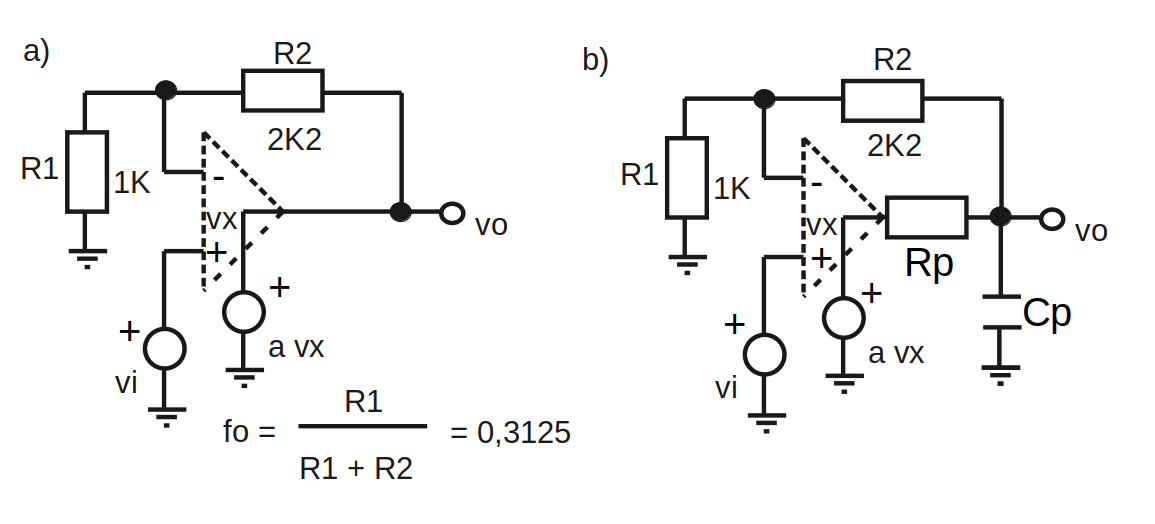
\includegraphics[width=4in]{figuras/estab11.png}\\
	\caption{Ejemplo de un amplificador de tensión realimentado de tres polos. a) Sin compensar
		y b) compensado por un polo dominante en $w_{pd}$. } \label{estab11}
\end{figure}

\begin{figure}
	\centering
	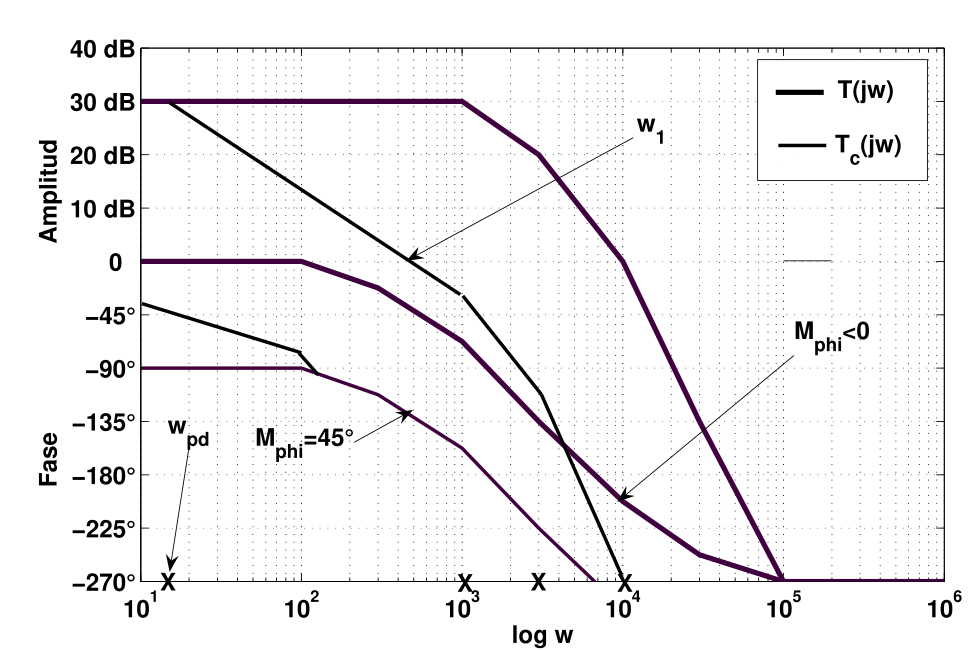
\includegraphics[width=5in]{figuras/estab12.png}\\
	\caption{Método gráfico de la compensación por polo dominante.}\label{estab12}
\end{figure}

Del gráfico de la figura \ref{estab12} se determina, en forma
aproximada, la frecuencia del polo dominante $w_{pd} \simeq 14,5
\quad rad/seg$. Una manera de implementar físicamente el polo
dominante es colocar un polo en $a(jw)$ (ver figura \ref{estab11}
b)). En estas condiciones la transferencia del amplificador sin
realimentar pasa a ser: $a(s)=\frac{\displaystyle 100}{\displaystyle
	(1+\frac{s}{1})(1+\frac{\displaystyle s}{\displaystyle
		3})(1+\frac{\displaystyle s}{\displaystyle 10})\displaystyle
	(1+\frac{s}{w_{pd}})}\quad$, con $w_{pd}=\frac{\displaystyle
	1}{\displaystyle R_p C_p}$. Para que el efecto de carga a la salida
no afecte al polo agregado ni a la ganancia sin realimentar $a_o$
debe ser $R_p \ll (R_1+R_2)$.

\subsection{Compensación por corrimiento del primer polo}

\hspace{10pt} Este método de compensación utiliza un concepto general similar al
caso de polo dominante; con la variante de desplazar al primer polo
de $T(jw)$ hacia frecuencias más bajas, de modo de convertirlo en
dominante. Para dar un ejemplo de este tipo de compensación se
utiliza el mismo sistema sin compensar del punto anterior es decir:
$T(s)=\frac{\displaystyle 31,6}{\displaystyle (1+\frac{\displaystyle
		s}{\displaystyle 1})(1+\frac{\displaystyle s}{\displaystyle
		3})(1+\frac{\displaystyle s}{\displaystyle 10})}\quad$. En la figura
\ref{estab13} se muestra, en línea gruesa, el sistema sin compensar;
en líneas más delgadas las distintas etapas de compensación. En
dicha figura se supone que se desea compensar para obtener un margen
de fase de $45°$. Los pasos realizados en el sistema de la figura
\ref{estab13} pueden resumirse en:
\begin{itemize}
	\item Se parte de los diagramas de Bode de $T(jw)$, línea
	gruesa. Allí se ve que el amplificador es inestable ($M\Phi<0$).
	\item Se utiliza la fase del sistema sin compensar para
	determinar la frecuencia $w_{1C1}$, esta frecuencia sería la
	frecuencia de $0 dB$ del sistema compensado para tener un margen
	de $45°$ ($\Phi(w_{1C1})=-135°)$. Esto se basa en la suposición que a dicha frecuencia
	la fase del sistema compensado coincide con la fase del sistema
	sin compensar.
	\item Se toma la frecuencia $w_{1C1}$ como frecuencia de $0 dB$
	del sistema compensado. Por lo tanto se traza el nuevo diagrama de
	amplitud de Bode a partir de dicha frecuencia  hacia la
	izquierda (en el ejemplo línea semi gruesa). El diagrama deberá trazarse con las pendientes
	adecuadas a la cantidad de singularidades encontradas a su
	izquierda. En este caso sólo actuará el polo desplazado, es
	decir la pendiente será de $-20 dB/dec$.
	\item Se tomará como frecuencia del polo desplazado a la
	frecuencia en que se intersectan $T_o$ con la pendiente trazada
	según los pasos del ítem anterior. En este caso será la
	frecuencia $w_{pc1}$.
	\item Con este polo desplazado se traza el nuevo diagrama de
	fase. Si a la frecuencia  $w_{1C1}$ dicha fase coincide con la
	fase del sistema sin compensar, ésta se toma como frecuencia final de
	corrimiento del primer polo. Si por el contrario no coincide,
	como en este ejemplo, se procede a realizar una nueva iteración
	(línea delgada) del método; utilizando como sistema sin compensar a $T_{C1}$. En
	este ejemplo en la segunda iteración finaliza la compensación,
	determinando que la frecuencia final de corrimiento será
	$w_{pc2}$.
\end{itemize}

\begin{figure}
	\centering
	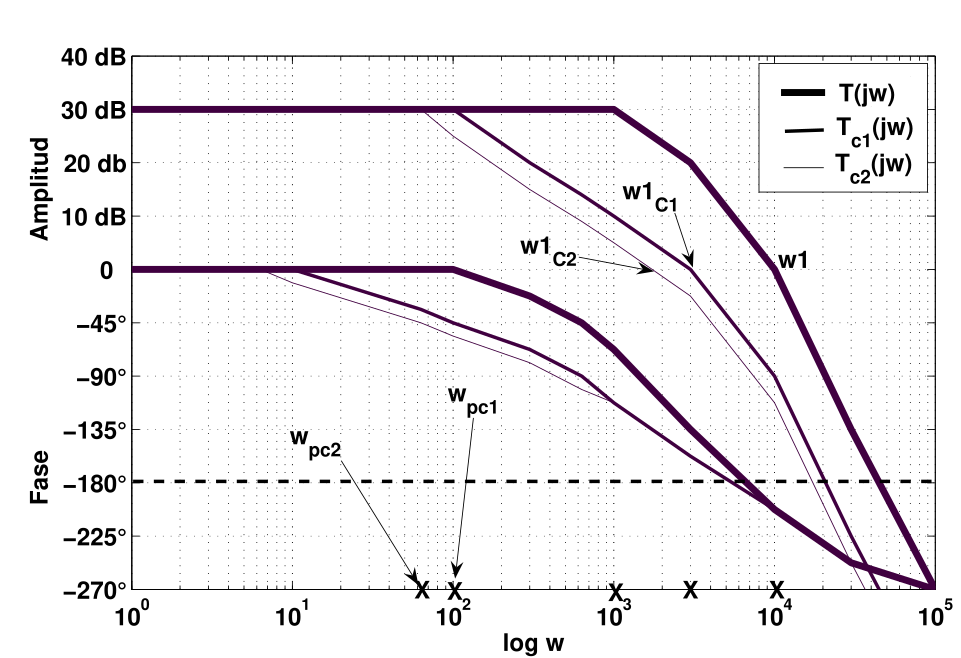
\includegraphics[width=5in]{figuras/estab13.png}\\
	\caption{Método gráfico de la compensación por corrimiento del primer polo.}\label{estab13}
\end{figure}

Para implementar físicamente este corrimiento debe identificarse
cual es el circuito determinante del primer polo. Por ejemplo en
amplificadores realizados con transistores bipolares (amplificadores
operacionales con tecnología bipolar), suele encontrarse ese primer
polo en una de las etapas amplificadoras en emisor común. Por lo
tanto el corrimiento de ese polo se logra colocando un capacitor
entre la base  y el colector del TBJ en cuestión. Tal compensación
es la que se suele realizar en los amplificadores operacionales
comerciales, tanto en los compensados internamente como en los que
deben ser compensados con la colocación de capacitores externos.

\subsection{Compensación por atraso de fase}

\hspace{10pt} Otro posible método de compensación de amplificadores realimentados
es el agregado en cascada de una red de atraso de fase a la ganancia
$a(jw)$ y por lo tanto a $T(jw)$. Esta red de atraso de fase se
compone de: un polo a la frecuencia $w_p$ y un cero a la frecuencia
$w_o$, de tal modo que $w_o>w_p$. Es decir que la ganancia de lazo
compensada sería: $T_c(s)=T(s)\frac{\displaystyle
	(1+\frac{\displaystyle s}{\displaystyle w_o})}{\displaystyle
	(1+\frac{\displaystyle s}{\displaystyle w_p})}$. Las frecuencias de
las singularidades agregadas se ubican de tal modo de lograr un
margen de fase determinado manteniendo la ganancia de lazo a
frecuencias bajas o medias del sistema original $T_o$.

Este método puede verse intuitivamente como similar al del
corrimiento del primer polo explicado en el punto anterior. Si se
diseña la frecuencia del cero de tal modo que sea igual a la
frecuencia del primer polo de $T(s)$, estas dos singularidades se
cancelarían; ubicando al polo de la red de atraso de fase a la
frecuencia calculada por el método de corrimiento del primer polo.

La transferencia de la red de atraso de fase puede verse en forma
cualitativa en la figura \ref{estab14}. El agregado de esta red
mantiene el valor de $|T(jw)|$ a frecuencias bajas y produce una
atenuación constante a frecuencias altas. Esta característica hace
que el pasaje por $0 dB$ de $|T_c(jw)|$ se realice a una frecuencia
menor que en el caso sin compensar; si aseguramos a esa frecuencia
el margen de fase requerido el sistema estaría entonces compensado.
La característica de fase de la red compensadora es tal que no
agrega fase adicional a frecuencias altas por lo que la condición
anterior puede ser cumplida.

\begin{figure}
	\centering
	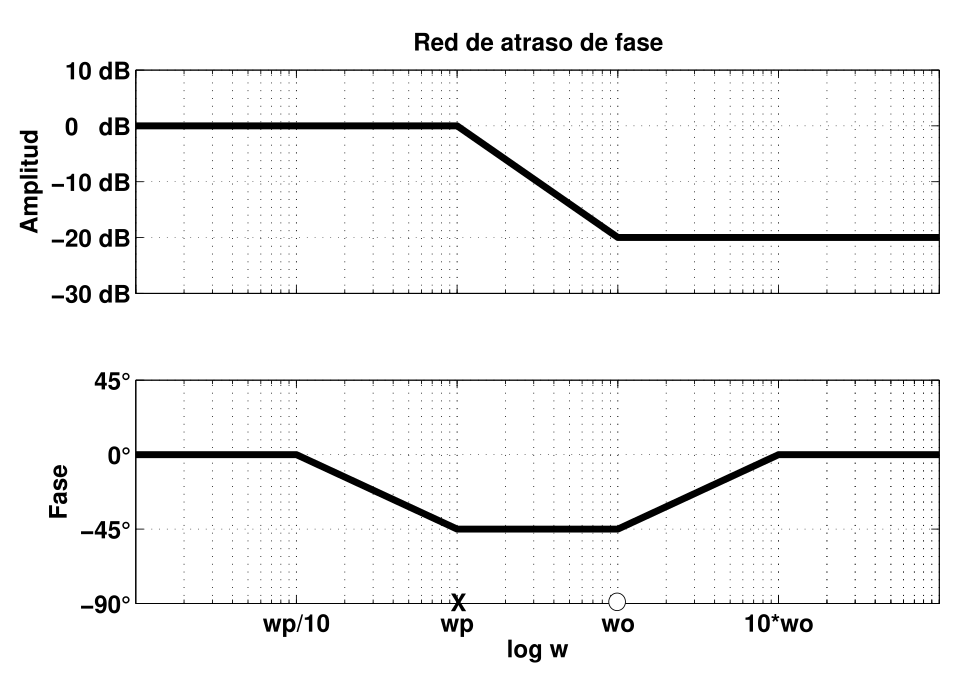
\includegraphics[width=5in]{figuras/estab14.png}\\
	\caption{Diagramas de Bode de la red de atraso de fase.}\label{estab14}
\end{figure}

Para explicar esta compensación utilizaremos el mismo ejemplo que en
los dos casos anteriores. En la figura \ref{estab15} se ubica al
cero de la red de atraso una década por debajo de la frecuencia en
que la fase original pasa por $-135°$; este criterio, algo
conservador, asegura que la fase original y la compensada coincidan
a dicha frecuencia  por lo tanto el margen de fase compensado será
$M\Phi=45°$. La frecuencia mencionada será la de $0 dB$ de
$|T_c(jw)|$. Como a la izquierda de dicha frecuencia habrá dos polos
(el primero original y el de la red de atraso) y un cero el diagrama
de amplitud deberá trazarse hacia la izquierda con una pendiente de
$-20 db/dec$, hasta que se encuentre con el primer polo original, a
partir de esa frecuencia el diagrama de amplitud será horizontal
hasta que se encuentre con el cero de la red de atraso; finalmente
volverá a tener una pendiente de $-20 dB/dec$ hasta intersectar a
$T_o$, siendo ésta la frecuencia del polo de la red de atraso.

\begin{figure}
	\centering
	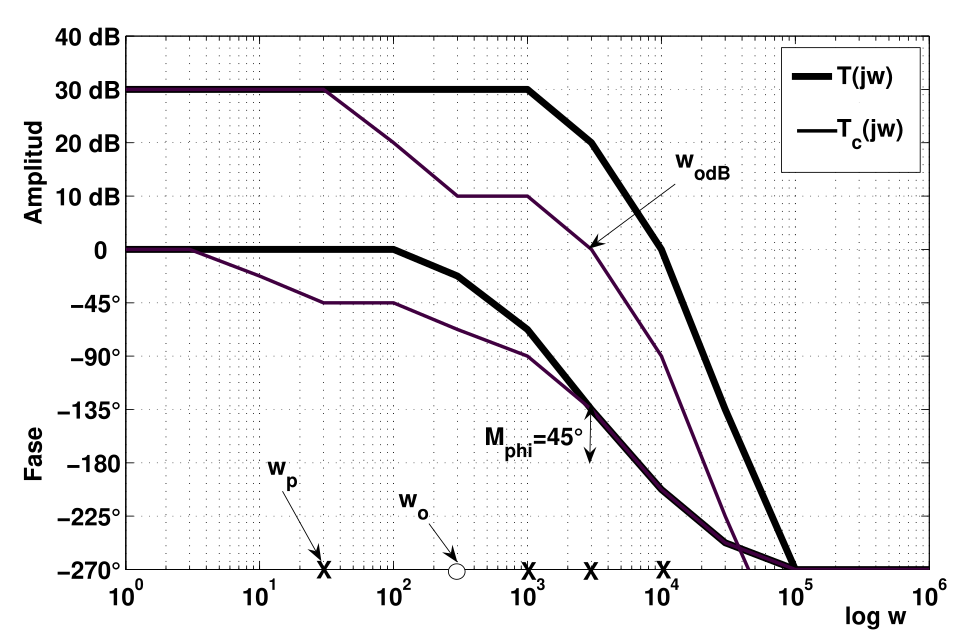
\includegraphics[width=5in]{figuras/estab15.png}\\
	\caption{Compensación por red de atraso de fase.}\label{estab15}
\end{figure}

Para implementar la compensación por atraso de fase utilizaremos un
circuito similar al de la figura \ref{estab11} a). En este caso se
agrega a $a(jw)$la red compuesta por $R_A$, $R_B$ y $C_B$, ver
figura \ref{estab16}.



\begin{figure}
	\centering
	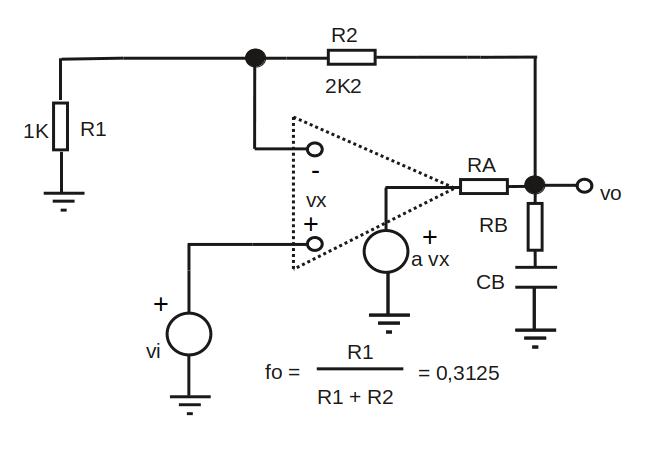
\includegraphics[width=4in]{figuras/estab16.png}\\
	\caption{Implementación de una compensación por atraso de fase.}\label{estab16}
\end{figure}

La transferencia de $T(jw)$ del amplificador compensado será:

\begin{center}
	
	$T_c(s)=\frac{\displaystyle 31,6}{\displaystyle
		(1+\frac{s}{1})(1+\frac{\displaystyle s}{\displaystyle
			3})(1+\frac{\displaystyle s}{\displaystyle 10})}\frac{\displaystyle
		(1+\frac{\displaystyle s}{\displaystyle w_o})}{\displaystyle
		(1+\frac{\displaystyle s}{\displaystyle w_p})}$
\end{center}



Con $w_o=\frac{\displaystyle 1}{\displaystyle C_BR_B}$ y
$w_p=\frac{\displaystyle 1}{\displaystyle C_B(R_A+R_B)}$.

En este caso en particular $w_o=300 \quad rad/seg$, $w_p=30 \quad
rad/seg$, $R_2=2K2$ y $R_1=1K$. Para que el efecto de carga de
salida no influya en $w_p$ ni en la ganancia sin realimentar $a_o$,
se debe asegurar que $R_A\ll(R_1+R_2)$. Bajo estas condiciones se
adopta $R_A\simeq 136 \Omega$, luego se calcula $R_B= 15 \Omega$ y
$C_B =220\mu F$.

\subsection{Compensación por adelanto de fase}

\hspace{10pt} El agregado de un cero a la ganancia de lazo $T(jw)$ a la frecuencia
$w_{0 dB}$, en que $|T(jw_{0 dB})|=1$; produce una mejora de $45°$
en el margen de fase en el sistema compensado. Esto se debe a que el
cero agregado aporta $+45°$ a la fase total a dicha frecuencia, sin
modificar apreciablemente el pasaje por $0 dB$ de $|T(jw)|$.

En general en un amplificador realimentado, agregar un cero en
$T(s)$ implica la ubicación de algún componente reactivo; esto
agrega además algún polo adicional a la transferencia. Si dicho polo
adicional se encuentra a una frecuencia mucho mayor que la
frecuencia del cero agregado, el cero producirá el efecto ya
explicado.

En este caso estamos agregando entonces, una red de adelanto de fase
con un cero en $w_o$ y un polo en $w_p$, tal que $w_o<w_p$; en la
figura \ref{estab17} se muestra los diagramas de Bode de una red de
adelanto de fase. La ganancia de lazo compensada será entonces:
$T_c(s)=T(s)\frac{\displaystyle 1+\frac{\displaystyle
		s}{\displaystyle w_o}}{\displaystyle 1+\frac{\displaystyle
		s}{\displaystyle w_p}}$.

\begin{figure}
	\centering
	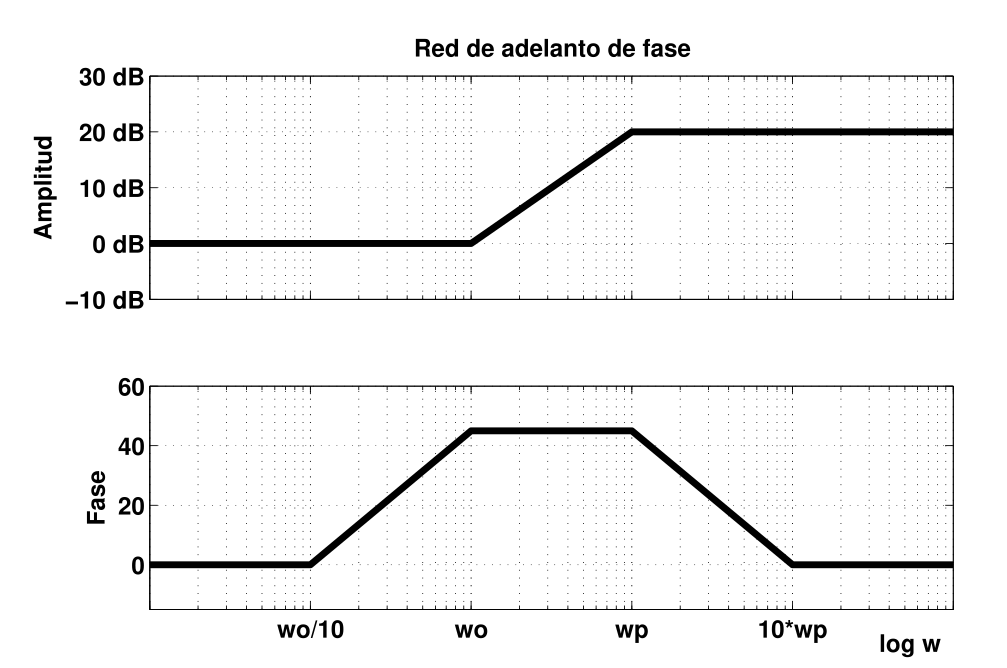
\includegraphics[width=5in]{figuras/estab17.png}\\
	\caption{Diagramas de Bode de la red de adelanto de fase.}\label{estab17}
\end{figure}

Para dar un ejemplo de este tipo de compensación utilizaremos el
circuito de la figura \ref{estab18}. En este circuito la ganancia
sin realimentar es: $a(s)= \frac{\displaystyle 110}{\displaystyle
	(1+\frac{\displaystyle s}{\displaystyle 1})(1+\frac{\displaystyle
		s}{\displaystyle 3})(1+\frac{\displaystyle s}{\displaystyle 10})}$
con $s$ en $ K\quad rad/seg$, el factor de realimentación (con
$C_2=0$) $f(s)=f_o=\frac{\displaystyle R_1}{\displaystyle R_1+R_2}$
y la ganancia de lazo sin compensar
$T(s)=a(s)f(s)=\frac{\displaystyle 10}{\displaystyle
	(1+\frac{\displaystyle s}{\displaystyle 1})(1+\frac{\displaystyle
		s}{\displaystyle 3})(1+\frac{\displaystyle s}{\displaystyle 10})}$.

\begin{figure}
	\centering
	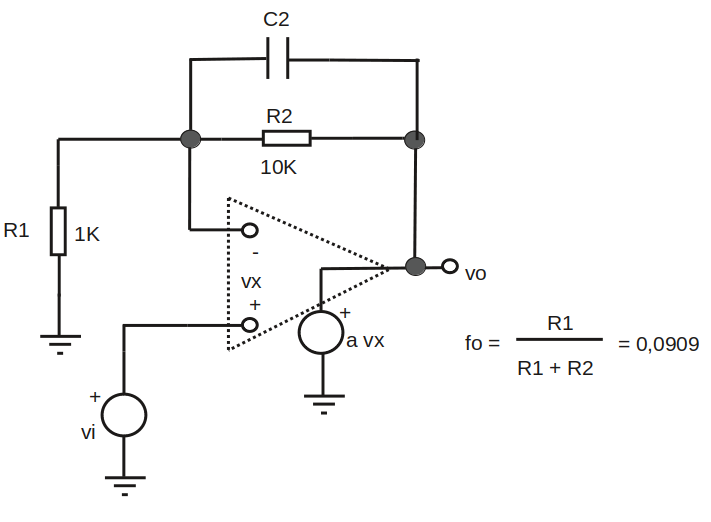
\includegraphics[width=4in]{figuras/estab18.png}\\
	\caption{Amplificador realimentado compensado por adelanto de fase.}\label{estab18}
\end{figure}

Si agregamos un capacitor $C_2$ en paralelo con $R_2$, la
transferencia de la red de realimentación pasará a ser: $f_c(s)=f_o
\frac{\displaystyle 1+\frac{\displaystyle s}{\displaystyle
		w_o}}{\displaystyle 1+\frac{\displaystyle s}{\displaystyle w_p}}$;
con $w_o=\frac{\displaystyle 1}{\displaystyle C_2R_2}$ y
$w_p=\frac{\displaystyle 1}{\displaystyle C_2R_1\parallel R_2}$,
con $w_o<w_p$ por lo que la red agregada será una de adelanto
de fase.

En la figura \ref{estab19} se muestran los diagramas de Bode de
amplitud y fase de la ganancia de lazo en ambos casos, no compensado
y compensado. En el primer caso se ve que el $M\Phi\approx0°$  y en
el caso compensado (suponiendo que agregamos un cero a la frecuencia
de $0 dB$) el margen de fase pasa a ser de aproximadamente $45°$. El
polo adicional agregado por la red de atraso está aproximadamente
una década por encima del cero, por lo que no influye
apreciablemente en el cálculo del margen de fase del amplificador
compensado.

\begin{figure}
	\centering
	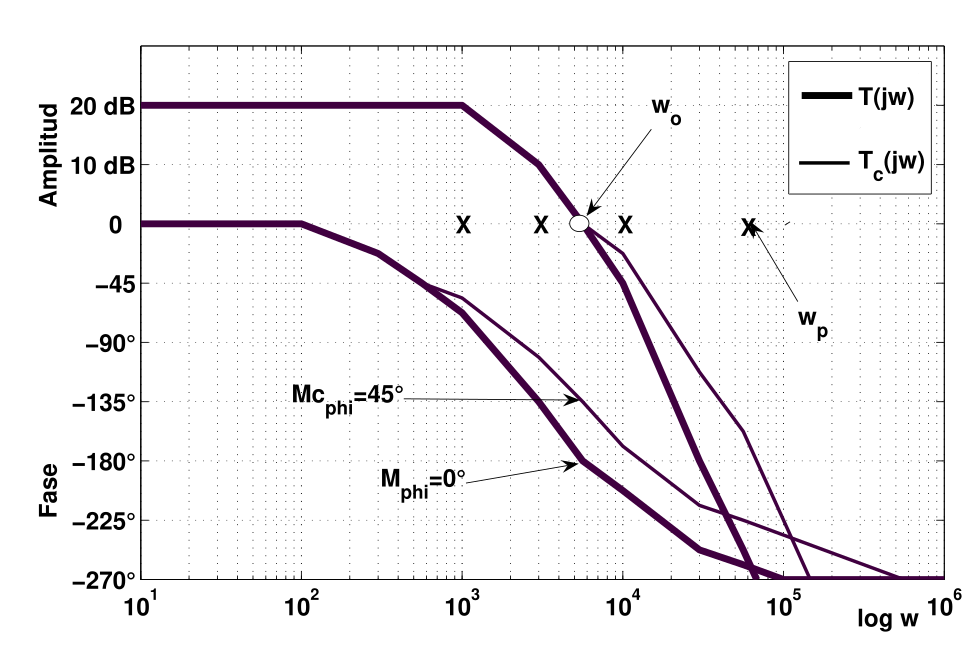
\includegraphics[width=5in]{figuras/estab19.png}\\
	\caption{Diagramas de Bode de la compensación por adelanto de fase.}\label{estab19}
\end{figure}

En este caso en particular el cero se establece a $w_o=5,62\quad
Krad/seg$, por lo tanto:

 $C_2=\frac{\displaystyle 1}{\displaystyle
	5620rad/seg\times10000\Omega}=17,8\quad nF$.
	
	El polo queda entonces
en:

$w_p=\frac{\displaystyle 1}{\displaystyle 17,8\quad nF\times 1K
	\parallel 10K}=61,8\quad Krad/seg$, más de una década por arriba del
cero.

Si se dispone, por mediciones, de la transferencia del amplificador
realimentado $A(jw)$, se puede establecer el criterio práctico para
realizar la compensación por adelanto de fase que consiste en
colocar el cero a la frecuencia en que la magnitud de la ganancia
realimentada pasa por un máximo. Este criterio práctico se basa en
el concepto que la frecuencia en la que se produce dicho máximo
coincide aproximadamente con la frecuencia en que $|T(jw)|=1$.

Para verificar el criterio volvamos a utilizar el amplificador sin
compensar de la figura \ref{estab18} con $(C_2=0)$. En la figura
\ref{estab21} se grafican en forma exacta los diagramas de Bode de
$T(jw)$ y de $A(jw)$. En el de $T(jw)$ se ve que los márgenes de
fase y ganancia son levemente positivos; también se verifica que la
frecuencia en que se produce el máximo valor en la magnitud de
$A(jw)$ coincide aproximadamente con la frecuencia de $0 dB$ de
$|T(jw)|$. Tomaremos del gráfico a $w_o\approx 5\quad Krad/seg$ como
frecuencia del cero que debemos agregar en la red de realimentación
para realizar la compensación. De tal modo $C_2=\frac{\displaystyle
	1}{\displaystyle 5000 \times R_2} \approx 20 \quad nF$; con este
valor de capacidad el polo adicional agregado estará en $w_p\approx
55 \quad Krad/seg$.

En la figura \ref{estab22} se muestra ahora los diagramas de Bode
de $T(jw)$ y de $A(jw)$ del sistema compensado. Se ve en ella que
los márgenes de fase aumentan considerablemente (lográndose la compensación buscada) y que el sobrepico
en la magnitud de $A(jw)$ es casi nulo.

\begin{figure}
	\centering
	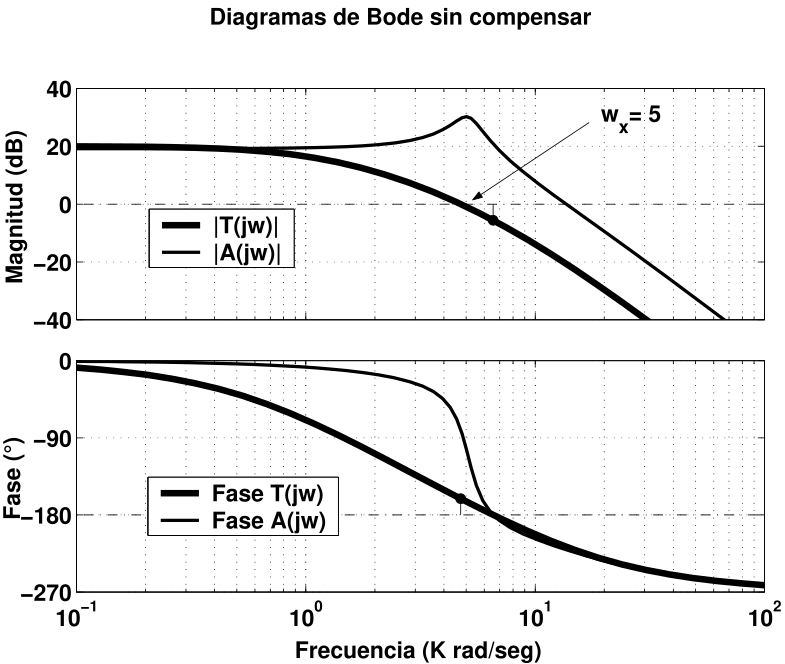
\includegraphics[width=5in]{figuras/estab21.png}\\
	\caption{Diagramas de Bode de $T(jw)$ y $A(jw)$ sin compensar.}\label{estab21}
\end{figure}

\begin{figure}
	\centering
	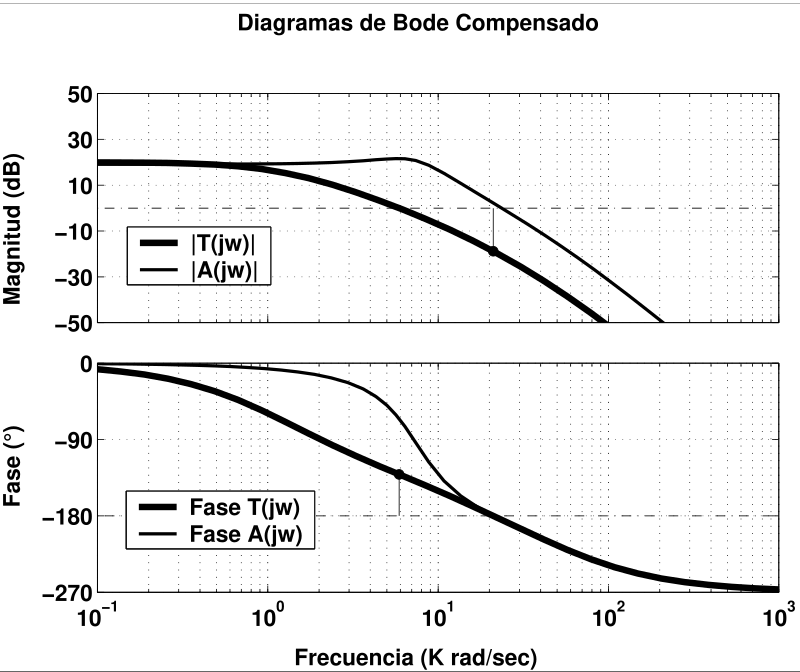
\includegraphics[width=5in]{figuras/estab22.png}\\
	\caption{Diagramas de Bode de $T(jw)$ y $A(jw)$ compensado por adelanto de fase.}\label{estab22}
\end{figure}

\section{Criterio de estabilidad de Routh}

\hspace{10pt} Otro método que puede ser utilizado para determinar la estabilidad
de un amplificador realimentado, es el criterio de Routh.

Este criterio matemático se basa en analizar las raíces de la
ecuación característica: $1+T(s)=0$. El criterio de Routh determina
la cantidad de raíces con parte real positiva que tiene un
polinomio.

Si se tiene un polinomio de grado $n$: $a_n s^n + a_{n-1} s^{n-1} +
a_{n-2} s^{n-2} + \cdots a_1 s+ a_0 = 0$, se procede a realizar el armado de la tabla de Routh, según lo mostrado en el cuadro \ref{tabla1}.

\begin{table}
	\centering
	\begin{tabular}{|l||c|c|c|c|}
		\hline
		&          &      &      &  \\
		$s^n$    & $a_n$         & $a_{n-2}$     & $a_{n-4}$     & $\cdots$ \\
		\cline{1-5}
		&          &      &      &  \\
		$s^{n-1}$  & $a_{n-1}$    & $a_{n-3}$     & $a_{n-5}$     & $\cdots$\\
		\cline{1-5}
		&          &      &      &  \\
		$s^{n-2}$ & $b_1$         & $b_2$     & $b_3$    & $\cdots$ \\
		\cline{1-5}
		&          &      &      &  \\
		$s^{n-3}$      & $c_1$         & $c_2$     & $\cdots$     & $\cdots$ \\
		\cline{1-5}
		&          &      &      &  \\
		$\cdots$      & $\cdots$         & $\cdots$     & $\cdots$    & $\cdots$\\
		\cline{1-5}
		&          &      &      &  \\
		$s^0$      & $k_1$         & $\cdots$     & $\cdots$    & $\cdots$\\
		\cline{1-5}
		\hline
	\end{tabular}
	\caption{Tabla de Routh de un polinomio de grado $n$.}\label{tabla1}
\end{table}

En la dos primeras filas de la tabla de Routh se disponen los
coeficientes del polinomio del modo mostrado en el cuadro
\ref{tabla1}. Las constantes $b_1$, $b_2$, $b_3$, etc, de la tercera
fila se calculan del siguiente modo:
\begin{eqnarray}
	\nonumber
	b_1 &=& \frac{\displaystyle a_{n-1} a_{n-2}-a_n a_{n-3}}{\displaystyle a_{n-1}} \\
	\nonumber
	b_2 &=& \frac{\displaystyle a_{n-1} a_{n-4}-a_n a_{n-5}}{\displaystyle a_{n-1}} \\
	\nonumber
	b_3 &=& \frac{\displaystyle a_{n-1} a_{n-6}-a_n a_{n-7}}{\displaystyle a_{n-1}}
\end{eqnarray}

Se completa la tercera fila hasta que dé cero alguno de los
coeficientes. Luego se forma la cuarta fila empleando las filas
segunda y tercera, las constantes son:
\begin{eqnarray}
	\nonumber
	c_1 &=& \frac{\displaystyle b_1 a_{n-3}-b_2 a_{n-1}}{\displaystyle b_1} \\
	\nonumber
	c_2 &=& \frac{\displaystyle b_1 a_{n-5}-b_3 a_{n-1}}{\displaystyle b_1} \\
	\nonumber
	c_3 &=& \frac{\displaystyle b_1 a_{n-7}-b_4 a_{n-1}}{\displaystyle b_1} \\
\end{eqnarray}

Se completa la cuarta fila hasta que dé cero alguno de los
coeficientes. Luego se forman las siguientes filas del mismo modo
con las dos filas superiores, hasta llegar a la fila correspondiente
a $s^0$. La distribución completa es triangular con las dos últimas
filas de un sólo componente.

Con esta tabla confeccionada el criterio de Routh dice que: el
número de raíces de la ecuación característica que tienen parte real
positiva es igual al número de cambios de signo de los coeficientes
de la primera columna, por lo tanto un sistema es estable si todos
los coeficientes de la primera columna son de igual signo.

Como ejemplo de cálculo se utilizará el amplificador del punto
\ref{ejemplo1}, es decir:


	\begin{equation}
		\nonumber
		T(s)=\frac{\displaystyle 31,6}{\displaystyle (1+\frac{\displaystyle
				s}{\displaystyle 1})(1+\frac{\displaystyle s}{\displaystyle
				3})(1+\frac{\displaystyle s}{\displaystyle 10})}
	\end{equation}





De $1+T(s)=0$ se obtiene $s^3+14s^2+43s+978=0$, por lo tanto la
tabla de Routh será la mostrada en el cuadro \ref{tabla2}. Allí se
ve que los coeficientes de la primera columna cambian dos veces de
signo, por lo tanto el polinomio tendrá dos raíces con parte real
positiva; es decir el amplificador realimentado será inestable.

\begin{table}
	\centering
	\begin{tabular}{|l||c|c|c|}
		\hline
		&          &      &        \\
		$s^3$    & $1$         & $43$     & $0$     \\
		\cline{1-4}
		&          &      &     \\
		$s^2$  & $14$    & $978$     & $0$     \\
		\cline{1-4}
		&          &      &        \\
		$s^1$ & $\frac{\displaystyle 14\times43-978\times1}{\displaystyle 14}=-26,86$         & $0$     & $0$     \\
		\cline{1-4}
		&          &      &        \\
		$s^0$      & $\frac{\displaystyle -26,86\times 978-14\times 0}{\displaystyle -26,86}=978$         & $0$       & $0$ \\
		\cline{1-4}
		\hline
	\end{tabular}
	\caption{Tabla de Routh ejemplo \ref{ejemplo1}.}\label{tabla2}
\end{table}

Otra posible aplicación del método de Routh es la de utilizarlo para
encontrar el límite de estabilidad. En el mismo ejemplo anterior
suponiendo una ganancia de lazo $T_o$ genérica, el polinomio
proveniente de la ecuación característica será:
$s^3+14s^2+43s+30(1+T_o)=0$, la nueva tabla de Routh es por lo tanto
la mostrada en el cuadro \ref{tabla3}.

\begin{table}
	\centering
	\begin{tabular}{|l||c|c|c|}
		\hline
		&          &      &        \\
		$s^3$    & $1$         & $43$     & $0$     \\
		\cline{1-4}
		&          &      &     \\
		$s^2$  & $14$    & $30(1+T_o)$     & $0$     \\
		\cline{1-4}
		&          &      &        \\
		$s^1$ & $\frac{\displaystyle 14\times43-30(\displaystyle 1+T_o)\times1}{14}$         & $0$     & $0$     \\
		\cline{1-4}
		&          &      &        \\
		$s^0$      & $30(1+T_o)$         & $0$       & $0$ \\
		\cline{1-4}
		\hline
	\end{tabular}
	\caption{Obtención del $T_o$ crítico a partir de la tabla de Routh.}\label{tabla3}
\end{table}

Como $T_o$ es siempre positivo (realimentación negativa), para que
no haya cambios de signo en la primera columna de coeficientes de la
tabla de Routh, se debe cumplir que: $\frac{\displaystyle
	14\times43-30(1+T_o)\times1}{\displaystyle 14}>0$, es decir que
$T_o<\frac{\displaystyle 14\times43}{\displaystyle 30}-1=19,07$ por
lo tanto el valor crítico será: $T_{oc}=19,07$.

\section{Lugar de raíces}

\hspace{10pt} El lugar geométrico de las raíces de la ecuación característica
según la variación de $T_o$, es una  herramienta importante para el
análisis y el diseño de amplificadores realimentados; ya que da una
idea acabada de la evolución de los polos del amplificador en
función del grado de realimentación que posean.

Su trazado exacto puede llegar a ser complejo debido al esfuerzo de
cómputo que conlleva su cálculo. Para su trazado pueden utilizarse
herramientas de \emph{software} tales como MatLab\circledR. Con la
herramienta \emph{rltool} de MatLab se trazó  (ver figura
\ref{estab23}) el lugar de raíces de la ecuación característica del
amplificador utilizado en el punto anterior. En dicha figura se
muestra que para $T_o=0$ el amplificador tiene los polos del
amplificador a lazo abierto, a medida que aumenta $T_o$ los polos se
van moviendo; acercándose primero y convirtiéndose en complejos
conjugados luego un par de ellos, y alejándose del origen hacia
$-\infty$ el restante. El par de polos complejos tienen en primera
instancia su parte real negativa, es decir el amplificador es
estable, hasta que $T_o$ llega al valor crítico; para $T_o>T_{oc}$
el amplificador es inestable.

\begin{figure}
	\centering
	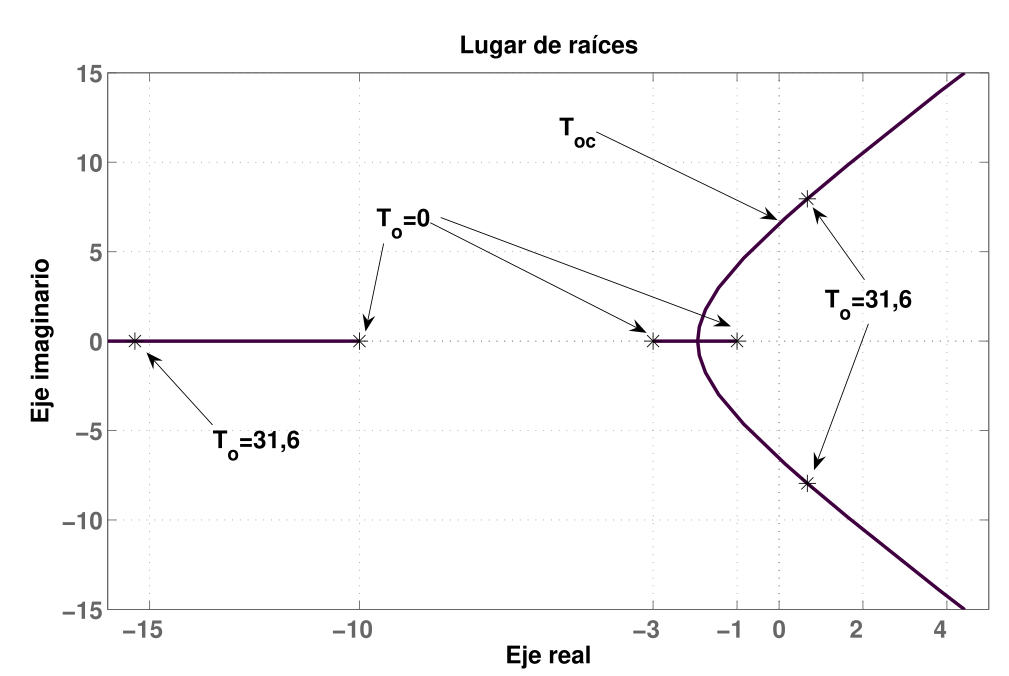
\includegraphics[width=5in]{figuras/estab23.png}\\
	\caption{Lugar geométrico de las raíces de un amplificador de tres polos.}\label{estab23}
\end{figure}

Existe un listado de reglas simplificado de trazado del lugar de
raíces, que ayuda a realizar un esquema cualitativo del mismo con un
esfuerzo de cálculo menor. Estas reglas permiten un trazado rápido
que sirve como ayuda conceptual en el diseño y en el análisis de los
amplificadores realimentados. Este esquema cualitativo puede servir
como complemento al método de Bode ya explicado del que se pueden
obtener resultados cuantitativos en forma gráfica.

El listado de reglas de trazado del lugar de raíces puede resumirse
en ocho reglas básicas:
\begin{enumerate}
	\item Las ramas del lugar de raíces de $1+T(s)$ comienzan en los
	polos de $T(s)$ ($T_o=0$, sin realimentación), y termina en los
	ceros de $T(s)$ donde $T_o \rightarrow \infty$, si $T(s)$ tiene
	más polos que ceros, alguna de las ramas del lugar geométrico de
	raíces terminará en infinito.
	\item   El lugar geométrico se sitúa a lo largo del eje real
	negativo siempre que exista un número impar de polos y ceros de $T(s)$ a su derecha contándolos hasta el origen.
	\item   Todos los segmentos del lugar geométrico que caen sobre
	el  eje real entre pares de polos (o entre pares de ceros) de
	$T(s)$ deben dividirse o ramificarse hacia fuera del eje real.
	Esta división deberá darse en un punto interno $\sigma_r$, denominado de
	ruptura.
	\item  El lugar geométrico es simétrico con respecto al eje
	real. Si existen raíces complejas, deberán existir sus
	conjugadas.
	\item Las ramas del lugar geométrico que se alejan del eje real
	la hacen con un ángulo recto con respecto a dicho eje.
	\item   Si las ramas del lugar geométrico se separan del eje
	real, lo hacen en un punto donde la suma de los vectores de las
	recíprocas de las distancias a los polos de $T(s)$ es igual a la
	suma de los vectores de las recíprocas de las distancias a los ceros de $T(s)$
	\item   Las ramas del lugar geométrico que terminan en el
	infinito lo hacen en forma asintótica. Dichas asíntotas son líneas rectas con
	ángulos con respecto al eje real dados por:
	$\alpha=\frac{\displaystyle (2n-1)\pi}{\displaystyle N_p-N_z}$, donde $N_p$ y $N_z$ son el número de
	polos y ceros de $T(s)$ y $n=0,1,\cdots,N_p-N_z-1$.
	\item   Todas las asíntotas de las ramas que terminan en
	infinito se cruzan en el eje real en un punto $\sigma_a$ dado
	por: $\sigma_a=\frac{\displaystyle \sum{[polos \quad de \quad T(s)]}-\sum{[ceros \quad
			de \quad T(s)]}}{\displaystyle N_p-N_z}$.
\end{enumerate}


Para dar un ejemplo de trazado se utilizará un amplificador de tres
polos con realimentación variable resistiva de modo que su ganancia
de lazo sea: $T(s)=\frac{\displaystyle T_o}{\displaystyle
	(1+\frac{\displaystyle s}{\displaystyle 1})(1+\frac{\displaystyle
		s}{\displaystyle 2})(1+\frac{\displaystyle s}{\displaystyle 4})}$.

Del criterio de Routh se establece que el valor crítico es
$T_{oc}=11,25$. En la figura \ref{estab24} se muestra el esquema del
lugar de raíces con los puntos salientes remarcados.

Por la \textbf{regla 1} para $T_o\rightarrow0$ el lugar comienza en
los polos de $T(s)$, es decir en $-1$, $-2$ y $-4$ y las tres ramas
terminarán en $\infty$ debido a que hay tres polos finitos y tres
ceros en $\infty$. Por la \textbf{regla 2} los segmentos del eje
real $[-\infty,-4)$ y $(-2,-1)$ pertenecen al lugar de raíces. Por
la \textbf{regla 3} las ramas que comienzan en $-2$ y $-1$ deben
separarse en un punto de ruptura interior $\sigma_r$ dado por la
ecuación de la \textbf{regla 6}: $\frac{\displaystyle
	1}{\displaystyle \sigma_r+1}+\frac{\displaystyle 1}{\displaystyle
	\sigma_r+2}+\frac{\displaystyle 1}{\displaystyle \sigma_r+4}=0$. Al
resolver esta ecuación cuadrática da $\sigma_{r,1}=3,22$ y
$\sigma_{r,2}=-1,45$, siendo esta última la solución posible ya que
pertenece al lugar de raíces (\textbf{regla 2}). Según la
\textbf{regla 7}, y teniendo en cuenta que $N_p-N_z=3$, los ángulos
de las asíntotas con el eje real serán:$\alpha=$ $+60°$, $-60°$ y
$180°$. Esta asíntotas se intersectarán en el punto:
$\sigma_a=\frac{\displaystyle (-1-2-4)-(0)}{\displaystyle 3}=-2,33$
dado por la \textbf{regla 8}.

Con estos cálculos y consideraciones se puede trazar en forma
aproximada el lugar geométrico de las raíces de las ecuación
característica (ver figura \ref{estab24}).

\begin{figure}
	\centering
	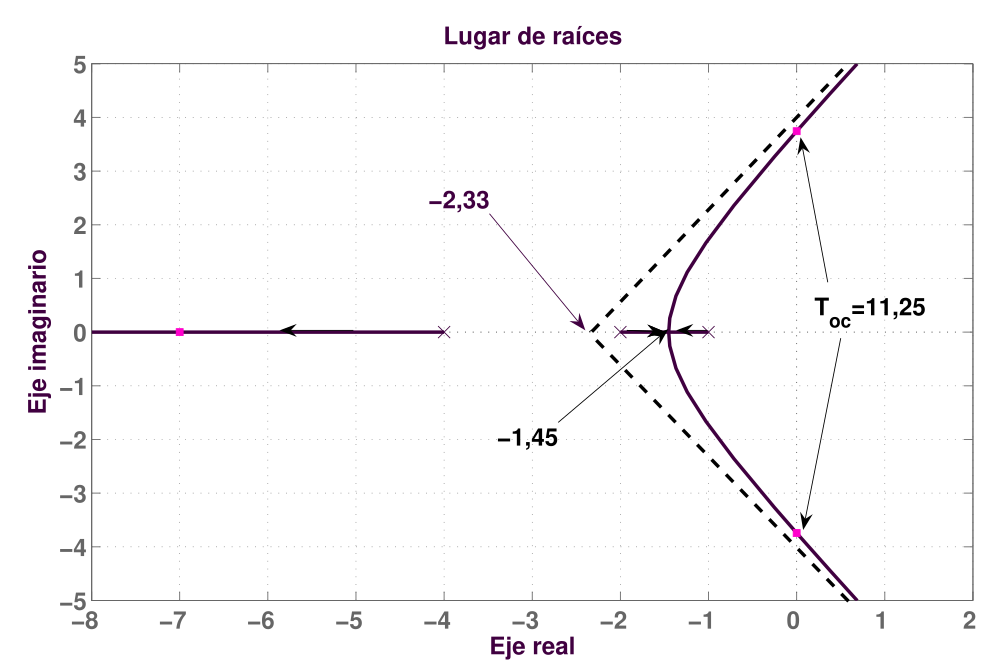
\includegraphics[width=5in]{figuras/estab24.png}\\
	\caption{Esquema del lugar geométrico de un amplificador de tres polos.}\label{estab24}
\end{figure}


Si a este mismo ejemplo se lo compensa agregándole un cero en
$s=-3$, adelanto de fase, la nueva ganancia de lazo será:
$T(s)=\frac{\displaystyle T_o(1+\frac{\displaystyle s}{\displaystyle
		3})}{\displaystyle (1+\frac{\displaystyle s}{\displaystyle
		1})(1+\frac{\displaystyle s}{\displaystyle 2})(1+\frac{\displaystyle
		s}{\displaystyle 4})}$, si suponemos que el polo adicional agregado
está a una frecuencia mucho mayor, y utilizando las reglas de
trazado del lugar de raíces; se tiene:

\begin{eqnarray}
	\nonumber
	\frac{\displaystyle 1}{\displaystyle \sigma_r+1}+ \frac{\displaystyle 1}{\displaystyle \sigma_r+2}+\frac{\displaystyle 1}{\displaystyle \sigma_r+4}&=& \frac{\displaystyle 1}{\displaystyle \sigma_r+3}\quad\quad \Longrightarrow \quad \sigma_r=-1,5344  \\
	\nonumber
	N_p-N_z &=& 2 \quad \Longrightarrow \quad \alpha = \pm 90° \\
	\nonumber
	\sigma_a &=& \frac{\displaystyle -1-2-4-(-3)}{\displaystyle 2}=-2
\end{eqnarray}

De estas reglas se puede trazar el lugar geométrico, observando que
el sistema es estable para cualquier valor de $T_o$. En la figura
\ref{estab25} se grafica dicho lugar geométrico.

\begin{figure}
	\centering
	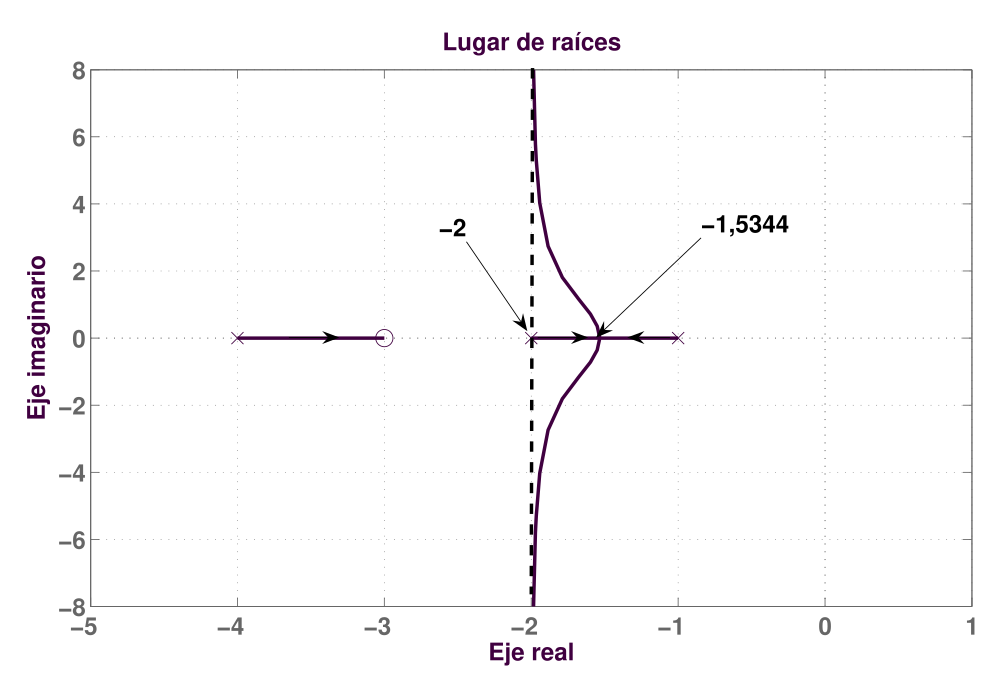
\includegraphics[width=5in]{figuras/estab25.png}\\
	\caption{Esquema del lugar geométrico de un amplificador de tres polos y un cero.}\label{estab25}
\end{figure}
